 \section{Preliminaries}

  We use ``iff\index{iff}'' as an abbreviation for ``if and only if.''
  We use set-theoretic concepts such as sets, relations and functions.
  For a set~$X$, $2^X$ denotes the powerset of $X$.
   $X\setminus Y$ denotes the subset of $X$ that consists of those
   elements of $X$ that are not elements of $Y$.
   Everywhere, we consider countably infinite set of logical formulae.
   A logic\index{logic} is a set of logical formulae, thus, there are at most
   $\powerset{\mathbb N}$ different logics once the set of logical
   formulae is fixed.
   Likewise, we consider at most countably many proofs and lambda terms.

   We denote partial maps as graphs.
   For example, $\{0\mapsto M, 1\mapsto N\}$ denotes a partial map that
   maps 0 to $M$ and 1 to $N$.
   We denote by $\dom(f)$ the domain of $f$, that is,
   the set of elements that are mapped to something.
   We also denote a partial map as a sequence whose index is the domain.
   For example, $(y_i)_{i\in I}$ denotes the partial map that maps
   $i\in I$ to $y_i$.
   For partial maps whose domains are disjoint, we use $\sqcup$ to
   denote the union.
   In other words, when $f$ and $g$ have disjoint domains, $f\sqcup g$
   denotes the
   partial map that maps $x$ to $f(x)$ or $g(x)$ when one of these is
   defined, or otherwise to nothing.

  We use BNF (Backus Naur Form) for giving inductive definitions for sets
  of sequents of symbols.
 \begin{example}[An example of BNF]
  When we say we define formulae~$\phi$ by BNF:
  \[
   \phi::= \bot \mid p\mid (\phi\imp\phi)
  \]
  where $p$ is a propositional variable, we actually define a set $\Phi$
  which is the smallest set such that
  \begin{itemize}
   \item $\bot$ is in $\Phi$
   \item each propositional variable is in $\Phi$ and
   \item if $\phi$ and $\psi$ are in $\Phi$, then $(\phi\imp\psi)$ is in $\Phi$.
  \end{itemize}
  and then we declare that we call elements of $\Phi$ formulae.
 \end{example}

 We take binary operators of the symbol $\imp$ or $\limp$,
 to be right associative.  For example, $\phi\limp\psi\limp\theta$
 is interpreted as $\phi\limp(\psi\limp\theta)$.

\section{History}

We briefly review the history of mathematical logic and computer science
to the extent relevant to the content of this thesis.
Especially, we focus on the treatments of Dummett's axiom $(a\imp
b)\lor(b\imp a)$ using the techniques in the history.
We confine ourselves to the developments of propositional logic and
ignore anything related to predicate logic or formalization of
mathematics.

\subsection{Birth of Formal Logic}

Implication is an important concept.
One treatment of implications called the material
implication\index{implication!material}.
The material implication can be traced back at least to
Frege's \textit{Begriffsschrift}~\citep{frege} in 1879.\index{Frege}
There, in the
section called ``conditionality,''
he begins by establishing four cases~\citep[p.~13]{frege}:
\begin{enumerate}
 \item $A$ is affirmed and $B$ is affirmed\,;
 \item $A$ is affirmed and $B$ is denied\,;
 \item $A$ is denied and $B$ is affirmed\,;
 \item $A$ is denied and $B$ is denied.
\end{enumerate}
Then he defines a notation involving $A$ and $B$
\[
\BGassert\BGconditional{B}{A}
\]
which ``stands for the
judgment that \textit{the third of these possibilities does not take
place, but one of the three other does\footnote{The emphasis is found in
the English translation~\citep[p.~14]{frege}.}}''~\citep[p.~14]{frege}.
In the contemporary common mathematical terminology, this is equivalent
to stating $B$ implies $A$.
It was Bertrand Russell who called this implication the material
implication,
according to~\citet{sep-conditionals}.
After his notation, we still use $\vdash$ for judgements in our formal
systems.
The view of logical formulae as graphical objects
will be inherited to proof nets (Section~\ref{sec:proofnets}).

\subsection{Intuitionistic Propositional Logic}

The intuitionistic propositional logic\index{logic!intuitionistic
propositional}\index{intuitionistic propositional logic|see{logic}} is a logic, that is, a set of
logical formulae.
Although the name ``intuitionistic'' comes from Brouwer's
intuitionism\index{intuitionism},
the original claims of intuitionism are unrelated to this thesis.
Brouwer\index{Brouwer} was skeptical about the value of formalization of
mathematics and considered the studies of formal axiomatized logic as
``mathematics of the second and third order''%
~\citep[p.~10]{stigt1998}.
Nontheless, Brouwer approved publication of his student Arend Heyting's
work on defining a set of logical formulae as the intuitionistic
propositional logic.

In 1930, Heyting~\cite{heyting1930}\index{Heyting} developed a deduction
system for the
intuitionistic propositional logic.  The presentation is similar to
the contemporary one except some notational differences.  The
logical connectives are the same $\{\wedge,\vee,\supset,\neg\}$ as today, the
first three binary and the last unary%
\footnote{Though, in this thesis, we prefer having nullary $\bot$ as a
primitive and define $\neg a$ as an abbreviation for $a\supset\bot$.}%
.  Logical formulae are constructed
using these connectives and the propositional variables.
Although he sometimes used parentheses, he still used more points
around outer connectives (e.g. $b\supset \kern -3pt\cdot \kern 2pt  a
\supset b$ indicates the left $\supset$ is outer and the right one is
inner), but we use parentheses here.
These formulae are axioms\footnote{The axioms with numberings are taken
from \citet{heyting1930}.}, i.e. assumed to be
``correct formulae''~\cite{heyting1930}\index{formula!correct}:
\begin{description}
 \item[2.1.] $a\supset (a\land a)$
 \item[2.11.] $(a\land b)\supset (b\land a)$
 \item[2.12.] $(a\supset b)\supset (a\land c)\supset (b\land c)$
 \item[2.13.] $((a\supset b)\land (b\supset c))\supset (a\supset c)$
 \item[2.14.] $b\supset (a\supset b)$
 \item[2.15.] $(a\land (a\supset b))\supset b$
 \item[3.1.] $a\supset (a\lor b)$
 \item[3.11.] $(a\lor b)\supset (b\lor a)$
 \item[3.12.] $((a\supset c)\land(b\supset c))\supset ((a\lor b)\supset
      c)$
 \item[4.1.] $\neg a\supset (a\supset b)$
 \item[4.11.] $((a\supset b)\land (a\supset \neg b)) \supset \neg a$\enspace.
\end{description}
There are more formulae given by the following rules~\cite{heyting1930}:
\begin{description}
 \item[1.2.] If $a$ and $b$ are correct formulas, then $a\land b$ is a correct
       formula\footnote{In quotes, we do not adjust the plural
      ``formulas'' and ``formulae.'' }.
 \item[1.3.] If $a$ and $b$ are correct formulas, then $b$ is a correct formula.
\end{description}

Following the intuitionists' belief
that ``it is in principle impossible to set up a system of formulas that
would be equivalent to intuitionistic mathematics, for the
possiblitities of thought cannot be reduced to a finite number of rules
set up in advance,''~\citep{heyting1930} he did not pursue completeness
results for the deduction system
except a remark mentioning Glivenko's
theorem~\citep{glivenko0,glivenko1}.
In other words, he did not pursue arguing that his system is strong
enough.
On the contrary, he argued his system is not too strong.
He used what would be called algebraic semantics today
in order to show that
each axiom is independent from the other axioms and that
the excluded middle is unprovable.
For example, in order to refute the excluded middle, he used the
following tables~\citep{heyting1930}:\\
 \begin{quotation}
 \begin{center}
  \begin{tabular}{c|ccc}
   $\supset $& 0  & 1  & 2 \\ \hline
   0 & 0 & 0 & 0 \\
   1 & 1 & 0 & 1 \\
   2 & 2 & 0 & 0
  \end{tabular}
  \hfill
  \begin{tabular}{c|ccc}
   $\wedge $& 0 & 1& 2\\ \hline
   0 & 0 & 1 & 2\\
   1 & 1 & 1 & 1\\
   2 & 2 & 1 & 2\\
  \end{tabular}
  \hfill
  \begin{tabular}{c|ccc}
   $\vee$& 0 & 1 & 2\\ \hline
   0 & 0 & 0 & 0 \\
   1 & 0 & 1 & 2 \\
   2 & 0 & 2 & 2\\
  \end{tabular}
  \hfill
  \begin{tabular}{c|ccc}
   $\neg $& 0 & 1 & 2\\ \hline
   & 1 & 0 & 1\\
  \end{tabular}\enspace.
 \end{center}
 \end{quotation}
When we assign one of $\{0,1,2\}$ to each propositional variable, we
can extend the assignment to all formulae using these tables.
For binary operators, the columns stand for the prearguments (the
arguments left of the operator) and the
rows stand for the postarguments (the arguments right of the operator).
For example, if we assign 1 to $a$ and 2 to $b$,
$a\supset b$ obtains value~0.
Under any assignment to propositional variables, all of Heyting's axioms
are assigned 0.  Moreover, these tables have two desirable properties:
\begin{enumerate}
 \item $0\land 0 = 0$
 \item $0\supset a$ has the value 0 only when $a = 0$.
\end{enumerate}
From these, all ``correct formulae'' in Heyting's deduction system
receive the value~0 under any assignments to propositional variables.
However, if we assign 2 to $a$, $(\neg \neg a)\supset a$
is assigned 2.  Thus, we can conclude that $\neg \neg a \supset a$ is
not a correct formula in Heyting's deduction system.
Note that the natural order between natural numbers
plays no rule here: it is not relevant that 2 is larger than 1 or 0 is
less than 1 (in other places he uses ``all positive and negative
whole numbers and 0'').  Although Heyting used natural numbers here, he
already obtained an equivalent notion of what is called Heyting algebra
today\footnote{Although he did not explicitly say that he can define a
partial order using the semantics for $\imp$.}.

We can refute Dummett's axiom $(a\supset b)\lor (b\supset
a)$\index{axiom!Dummett's} in the same method.
Indeed, according to the tables below, when we assign 1 to $a$ and 2
to $b$, $(a\supset b)\lor (b\supset a)$ obtains 4, which is not 0.
Since all correct formulae receive 0, $(a\imp b)\lor (b\imp a)$ is not a
correct formula.
 \begin{center}
  \begin{tabular}{c|ccccc}
   $\imp$ & 0& 1& 2& 3& 4\\ \hline
   0& 0& 0& 0& 0& 0\\
   1& 1& 0& 1& 0& 1\\
   2& 2& 2& 0& 0& 2\\
   3& 3& 3& 3& 0& 3\\
   4& 4& 0& 0& 0& 0
  \end{tabular}
  \hfill
  \begin{tabular}{c|ccccc}
   $\wedge$& 0& 1& 2& 3& 4\\ \hline
   0 & 0& 1& 2& 3& 4\\
   1& 1& 1& 3& 3& 1\\
   2& 2& 3& 2& 3& 2\\
   3& 3& 3& 3& 3& 3\\
   4& 4& 1& 2& 3& 4\\
  \end{tabular}
  \hfill
  \begin{tabular}{c|ccccc}
   $\vee$&0 &1 &2 &3 &4 \\ \hline
   0& 0& 0& 0& 0& 0\\
   1& 0& 1& 4& 1& 4\\
   2& 0& 4& 2& 2& 4\\
   3& 0& 1& 2& 3& 4\\
   4& 0& 4& 4& 4& 4\\
  \end{tabular}
  \ruleskip
  \begin{tabular}{c|ccccc}
   $\neg$& 0& 1& 2& 3& 4\\ \hline
   & 3& 3& 3& 0& 3\\
  \end{tabular}
 \end{center}

\subsubsection{G\"odel}
In 1932, G\"odel published a short note~\cite{godelprop} on
intuitionistic propositional
logic, where he proved two theorems: that the intuitionistic propositional logic
cannot be seen as a many-valued logic and that
there are infinitely many propositional logics between the
intuitionistic propositional logic and the ``ordinary'' (in today's
terminology, classical) propositional logic.  The second result is the
first contribution to the realm of intermediate
logics\index{logic!intermediate} (according to Troelstra~\cite[p.~223]{goedelcollected}).
For distinguishing those intermediate logics and the intuitionistic
propositional logic, he uses a formula~$F_n$ for each positive natural
number~$n$:
\[
 F_n = \bigvee_{1\le i < k\le n}\left((a_i\supset a_k) \land (a_k\supset a_i)\right)\enspace.
\]
On an $n$-element chain, $F_{n+1}$ is valid while $F_n$ might not be
satisfied.  As a result, no $F_n$ is valid in the intuitionistic
propositional logic.

Among the formulae~$F_n$,
especially, the formula~$F_2$, which is $(a_1\supset a_2)\land (a_2\supset
a_1)$, brings contradiction into classical or intuitionistic logic.  If we
had $(p\land q)\supset p$ and $F_2$ as theorems in a logic closed under
substitution and modus ponens,
$a_1\supset a_2$ is also a theorem and all formulae would be theorems or
there would be no theorems.
% In Chapter~\ref{ch:exchange} we investigate a logic with an axiom similar to $F_2$:
% $(\phi\limp\psi)\otimes(\psi\limp\phi)$, where $\otimes$ is the
% multiplicative conjunction and $\limp$ is the linear implication.  Such
% attempt has been made possible by the development of linear and
% substructural logics explained below in \ref{linear}.
In short, in some of those settings, $(p\otimes q)\limp p$ is
not a theorem because we are not allowed to throw away $q$.

In the final sentence, \citet{godelprop} states what is known as
disjunction property\index{disjunction property} today%
\footnote{Disjunction property can be proved by soundness and
completeness with respect to Kripke models.  There is another, syntactic
technique called Aczel's slash~\citep[Ch.~3. 5.7.]{troelstra1988constructivism}.}: ``besides, the
following holds with full
generality: a formula of the form $A\lor B$ can only be provable in $H$
if either $A$ or $B$ is provable in $H$,'' where $H$ is Heyting's calculus.
According to this statement, it is obvious that Dummett's axiom
$(p\supset q) \lor (q\supset p)$ is not provable.

Although Troelstra~\cite[p.~223]{goedelcollected} writes ``the reasons
for studying intermediate logics are mainly technical,'' we find that
one typical intermediate logic, G\"odel--Dummett logic, has a
computational interpretation which has already been known: waitfreedom.
The connection between G\"odel--Dummett logic and waitfreedom will be
treated in Chapter~\ref{ch:lambda}.

\subsection{The Brouwer--Heyting--Kolmogorov Interpretation of Logical Connectives}

\subsubsection{Kolmogorov's view of implication as problem reduction}

Thanks to Heyting~\cite{heyting1930}, we have a formal
characterization of the intuitionistic implication.
In 1932, Kolmogorov~\cite{kolmogorov1932} introduced a ``calculus of problems''
that coincides with the intuitionistic propositional logic.
In the calculus of problems, the logical connectives $\vee, \wedge,
\supset$ connect problems together to form another problem.
 \begin{quote}
  If $a$ and $b$ are two problems, then $a\land b$ designates the
  problem ``to solve both problems $a$ and $b$,'' while $a\lor b$
  designates the problem ``to solve at least one of the problems $a$ and
  $b$.''  Furthermore, $a\supset b$ is the problem ``to solve $b$
  provided that the solution for $a$ is given'' or, equivalently, ``to
  reduce the solution of $b$ to the solution of
  $a$.''  \ldots $\neg a$ designates the problem ``to obtain a
  contradiction provided that the solution of $a$ is
  given.''~\cite[p.~329]{kolmogorov1932}
 \end{quote}
 Here, the intuitionistic implication\index{implication!intuitionistic}
 is explained as reduction of problems.
 He continues to validate Heyting~\cite{heyting1930}'s axioms, and the
 deduction rules with respect to the problem calculus interpretation.

 Furthermore, he finds a reason for not including the law of excluded
 middle $a\lor \neg a$ by saying ``one must possess a general method
 either to prove or to reduce to a contradiction any proposition.  If
 our reader does not consider himself to be omniscient, he will probably
 determine that the formula cannot be found on the list of problems
 solved by him''~\cite{kolmogorov1932}.
 This argument is enough to reject Dummett's axiom $(a\supset b)\lor
 (b\supset a)$ because one must possess a general method, given any two
 problems, to
 determine whether
 one problem can be reduced to the other or the other way around.
 For the computational meaning of the law of excluded middle, we have to
 wait until 1990's.
 And the computational interpretation of Dummett's axiom is
 presented in Chapter~\ref{ch:lambda} in this thesis.

\subsubsection{Realization as Typed Lambda Terms}

One formulation of the
Brouwer--Heyting--Kolmogorov\index{Brouwer--Heyting--Kolmogorov
interpretation}
(BHK\index{BHK|see{Brouwer--Heyting--Kolmogorov interpretation}})
interpretation reads: ``a proof of the
implication $\varphi\supset\psi$ is a construction which permits us to
 transform any proof of $\varphi$ into a proof of $\psi$''~\cite[Ch.~1, 3.1.]{troelstra1988constructivism}.
The BHK
interpretation does not specify what is a proof or what kind of
transformation witnesses implication.


\subsection{Natural Deduction and Sequent Calculus}

\subsubsection{Gentzen's Deduction Systems}\index{Gentzen}

The deduction system of \citet{heyting1930} characterizes what is still
called intuitionistic propositional logic today. However, Heyting's
system has one drawback, which is shared with almost all%
\footnote{Even Hilbert-style deduction
systems can avoid this drawback if all theorems are axioms.} other
Hilbert-style derivation systems:
in order to prove a logical formula, sometimes we have to
mention a larger, more complicated formula.  Actually, there
are alternative formulations of intuitionistic (and classical)
propositional logic by \citet{gentzen} where we only have to
mention subformulae of the formula being proven.
The desirable property is called subformula property\index{subformula property}.
The two proof systems are called natural deduciton\index{natural
deduction} and sequent calculus\index{sequent calculus}.

In contrast to the sytem of \citet{heyting1930} where a proof yields a
finite set of ``correct formulae,'' a proof in natural deduction and
sequent calculus yields a pair of assumptions and conclusions.
\citet{gentzen} used the form
\[
 \mathbf{A_1},\ldots,\mathbf{A_{\boldsymbol\mu}}\longrightarrow \mathbf{B}
\]
as a sequent.  We will use $\vdash$ instead of $\longrightarrow$.
In any case, a sequent stands for the implication:
the conjunction of $\mathbf{A_i}$'s implies $\mathbf{B}$.

In natural deduction, the assumptions and conclusions are presented
vertically.  For example,
 \begin{center}
  \AxiomC{$A\land B$}
  \UnaryInfC{$B$}
  \DisplayProof
 \end{center}
 has a single assumption $A\land B$ and a conclusion~$B$.
 The same content can be shown as
  \begin{center}
   \AxiomC{}
   \UnaryInfC{$A\land B\tr A\land B$}
   \UnaryInfC{$A\land B\tr B$}
   \DisplayProof\enspace.
  \end{center}
 The horizontal line shows an application of an inference rule%
 \footnote{In \citep{gentzen}, an inference rule is called an inference
 figure schema.}.
 The sequent on top of the inference rule is called the
 \textit{assumption}\index{assumption} of
 the rule and the sequent below is called the
 \textit{conclusion}\index{conclusion} of the rule.
Natural deduction has \textit{introduction rules}\index{introduction
 rule}
 and \textit{elimination rules}\index{elimination rule} for each
logical connectives.  An introduction rule of a connective contains the
 connective in the conclusion but not in the assumptions (if any).
 An elimination rule of a connective contains the connective in one of the
 assumptions but not in the conclusion.
For example, the introduction and elimination
rules for $\wedge$
 (conjunction\footnote{\citet{gentzen} and \citet{prawitz1965} used
 $\&$.}) is as follows:
  \begin{center}
   \AxiomC{$\G\tr\phi$}
   \AxiomC{$\G\tr\psi$}
   \BinaryInfC{$\G\tr\phi\land\psi$}
   \DisplayProof
   \hfill
   \AxiomC{$\G\tr\phi\land\psi$}
   \UnaryInfC{$\G\tr\phi$}
   \DisplayProof
   \hfill
   \AxiomC{$\G\tr\phi\land\psi$}
   \UnaryInfC{$\G\tr\psi$}
   \DisplayProof
   \enspace.
  \end{center}
  These rules are the meaning of conjunction~$\wedge$.
  In sequent calculus, the introduction rules stay the same but called
  the right rules because they operate on the right hand side of
  sequents.
  The elimination rules are rewriten so that they operate on the left
  side of sequents and they are called the left rules.

  In Chapter~\ref{ch:exchange}, we will use hypersequent calculus for
  presenting Abelian logic.
  In Chapter~\ref{ch:lambda}, we will use hypersequent-stye natural deduction
  for preseinting G\"odel--Dummett logic.

\subsubsection{Prawitz's Analysis of Natural Deduction}

\citet{gentzen} did not prove the subformula property immediately for
natural deduction.  He proved the subformula property for sequent
calculus first and then after that obtained the property of natural
deduction as a corollary.
On the other hand, \citet{prawitz1965} studied natural deduction in
itself.

Inversion principle states that an occurrence of a logical connective
in a proof can be removed when the connective is introduced by
an introduction rule, and then immediately below, eliminated by an
elimination rule.  A logical formula occurrence containing such a
connective is called a maximal formula.
For example, for conjunction, a natural deduction
derivation~\citep[p.~36]{prawitz1965} can be reduced
 \begin{center}
  from
 \AxiomC{$\Sigma_0$}
  \UnaryInfC{$A$}
 \AxiomC{$\Sigma_1$}
  \UnaryInfC{$B$}
  \LL{$\wedge\intro$}
  \BinaryInfC{$A\land B$}
  \LL{$\wedge\elim$}
  \UnaryInfC{$A$}
  \DisplayProof
  to
 \AxiomC{$\Sigma_0$}
  \UnaryInfC{$A$}
  \DisplayProof
 \end{center}
 where $\Sigma_0$ and $\Sigma_1$ stand for derivations with conclusions
 $A$ and $B$ respectively.
 In the reduction, the occurrence of $\wedge$ is removed.
 The same holds for other logical connectives: thus we can remove
 maximal formulae.

 Further, \citet[Chapter~IV]{prawitz1965} formulated a weaker notion
 called maximal segments.
 Above, in the definition of maximal formulae,
 the elimination rule must be placed immediately below the corresponding
 introduction rule.  Prawitz allowed other inference lines between the
 introduction and elimination rules and defined maximal segments%
 \footnote{A maximal segment can contain many occurrences of the same
 formula without being influenced by any inference rules.
 Such ``syntactic beaurocracy'' can be removed by proof nets.
 See Section~\ref{sec:proofnets} for an example.}.
 A derivation without maximal segments is called normal.
 And Prawitz proved the existence of a normal derivation of $\G\vdash A$
 given any derivation of $\G\vdash A$.
 \citet{prawitz1965} treated first-order, second-order and modal logics but
 we do not elaborate.

 The reductions and the normal form coincide with the $\beta$-reduction
 and the normal form in the typed lambda
 calculi under Curry--Howard isomorphism.

\subsubsection{Prior's Tonk}

\citet{prior60} invented a logical connective called tonk.
 \begin{center}
\AxiomC{$\phi$}
\UnaryInfC{$\phi \text{ tonk }\psi$}
\DisplayProof
  \hfill
\AxiomC{$\psi$}
\UnaryInfC{$\phi \text{ tonk }\psi$}
\DisplayProof
  \hfill
\AxiomC{$\phi\text{ tonk }\psi$}
\UnaryInfC{$\phi$}
\DisplayProof
  \hfill
\AxiomC{$\phi\text{ tonk }\psi$}
\UnaryInfC{$\psi$}
\DisplayProof
 \end{center}
From this,
inversion principle requires this reduction:
 \begin{center}
  from
  \AxiomC{$\phi$}
  \UnaryInfC{$\phi\text{ tonk }\psi$}
  \UnaryInfC{$\psi$}
  \DisplayProof
  to
  \AxiomC{$\phi$}
  \UnaryInfC{$\psi$}
  \DisplayProof\enspace.
 \end{center}
The reduct is considered nonsense because if there are any theorems all
formulae must be theorems.  This is an argument refuting the tonk operator.
However, in Chapter~\ref{ch:exchange},
we pursue the possibility of compensating the
nonsense by the dual nonsense, namely:
 \begin{center}
  \AxiomC{$\phi\qquad \psi$}
  \UnaryInfC{$\psi\qquad \phi$}
  \DisplayProof\enspace.
 \end{center}
 Prior's paper is titled ``the runabout inference-ticket.''
 In Chapter~\ref{ch:exchange}, we are going to consider the roundtrip
 inference-ticket.


\subsection{Curry--Howard Isomorphism}

At the core of computer science lies the interplay of static formalism
and dynamic behaviour.  We can find examples in typed lambda calculi,
where static formalism of type derivations interacts with dynamic
behaviour of lambda terms.
Type derivations of static objects associtating lambda terms to types.
The reduction on terms gives dynamics, defining which term reduce
to which.  Static type derivations can guarantee dynamic properties of
programs such as strong normalization~\citep{girard1989proofs} and more
specific properties using parametricity arguments~\citep{reynolds1983types}.

The Curry--Howard isomorphism~\index{Curry--Howard isomorphism}
is originally a correspondence between
intuitionistic propositional logic proofs and typed lambda terms, but
the technical term has obtained a more general meaning spanning over the
correspondence between proofs and programs in general.
The phrase ``computational interpretation'' is most often used for
the Curry--Howard
isomorphism~\citep{abramsky1993computational,parigot2000,bierman1998,martini1996}.
\citet{curryhoward} recently presented a comprehensive reference book on the
topic, containing lots of historical and bibliographical remarks.

\subsubsection{Curry's Discovery}
The Curry--Howard isomorphism is originally the correspondence of
the typed lambda terms and the proofs of the implicational fragment%
 \footnote{The implicational fragment\index{fragment!implicational} of a
 logic can be defined by taking formulae only containing implications
 but no other connectives.} of
the intuitionistic propositional logic.
According to \citep{curryhoward}, the first explicit statement of the
correspondence appears
in the retiring presidential address to the Association for Symbolic
Logic titled ``the combinatory foundations of mathematical
logic''~\cite{curry1942}\index{Curry}.
The footnote~28 of \citep{curry1942} reads:
 \begin{quote}
  Note the similarity of the postulates for $F$ and those for $P$.  If
  in any of the former postulates we change $F$ to $P$ and drop the
  combinator we have the corresponding postulate for $P$
 \end{quote}
 where a postulate for $F$ is is something like $\tr F X Y f$ which
 represents the statement that $f$ belongs to the
 class of functions from $X$ to $Y$; and $P$ is the implicational
 fragment of the intuitionistic propositional logic.
 On the same page, there is Postulate~(PC):
\[
 \vdash (\beta\supset (\alpha\supset \gamma))\supset (\alpha \supset
 (\beta\supset \gamma))
\]
and the corresponding Postulate~(FC):
\[
 \vdash F(F\beta(F\alpha\gamma))(F\alpha(F\beta\gamma))C
\]
 where $C$ is $\lambda^3 xyz\cdot xzy$ and the notation $F\alpha\beta$
 shows the
 functional character of a
 function from $\alpha$ to $\beta$.  The postulate~(FC) is said to
 state the functional character of $C$.
 In this thesis, we use sequent style natural deduction system so that these
 postulates can be derived as
 \[
 \AxiomC{}
 \useq{\tj{x}{\beta\supset (\alpha\supset \gamma)}}{\tj{x}{\beta\supset
 (\alpha\supset \gamma)}}
 \AxiomC{}
 \useq{\tj{z}{\beta}}{\tj{z}{\beta}}
 \bseq{\tj{x}{\beta\supset (\alpha\supset \gamma)},
 \tj{z}{\beta}}{\tj{xz}{\alpha\supset\gamma}}
 \AxiomC{}
 \useq{\tj{y}{\alpha}}{\tj{y}{\alpha}}
 \bseq{\tj{x}{\beta\supset (\alpha\supset \gamma)},
 \tj{z}{\beta},\tj{y}{\alpha}}{\tj{xzy}{\gamma}}
 \useq{\tj{x}{\beta\supset (\alpha\supset
 \gamma)},\tj{y}{\alpha}}{\tj{\lambda z. xzy}{\beta\supset\gamma}}
 \useq{\tj{x}{\beta\supset (\alpha\supset
 \gamma)}}{\tj{\lambda y.\lambda z. xzy}{\alpha\supset(\beta\supset\gamma)}}
 \useq{}{\tj{\lambda x.\lambda y.\lambda z. xzy}{{(\beta\supset (\alpha\supset
 \gamma))}\supset (\alpha\supset(\beta\supset\gamma))}}
 \DisplayProof \enspace .
 \]
 Indeed, the last sequent associates the term $\lambda x.\lambda
 y.\lambda z. xzy$, which is the combinator $C$, to the logical formula
 $(\beta\supset (\alpha\supset
 \gamma))\supset (\alpha\supset(\beta\supset\gamma))$.
 Throughout this thesis, we use $\colon$ to associate terms with types.

 Henceforth, we do not give deduction system of a logic and
 typing rules for a typed lambda calculi separately because
 the former can be obtained from the lattar by this correspondence.
The
precise statements for the correspondence appear in
\citet[9E]{curry1974combinatory}, a section titled ``analogies with
propositional algebra.''

Curry--Howard isomorphism provides
one realization of BHK interpretation: proofs as lambda terms where the
introduction rule of implication is realized as the lambda abstraction
and the elimination rule of implication is realized as the application
of lambda terms.
This encoding has a desirable property:
the reductions in the lambda calculus corresponds to the reductions of
proofs that
removes detours.
For example, suppose a natural deduction proof introduces an implication and then
immidiately eliminate the
implication.  This proof can be encoded as a lambda term whose outermost
structure is a $\beta$-redex: $(\lambda x. M)N$.
 The result of the $\beta$-reduction $M[N/x]$ encodes a proof tree using
 the same assumptions as the original and concluding the same formula as
 the original, yet without the aforementioned detour.
 a proof of implication allows transformation of proofs
by means of
substitution.  The encoding of proofs as lambda terms is traditionally
called the Curry--Howard isomorphism.
% The situation is similar to axiomatized geometry where lines and points
% could be tables and chairs \fix{(cite)}.
The former explanation of implications is justified in classical propositional logic.
The latter view is most naturally materialized in the situation of
intuitionistic propositional logic.  The last century saw their
generalization called intermediate logics~\citep{umezawa} (or superintuitionistic
logics\index{logic!superintuitionistic}), of which a typical example is
called G\"odel--Dummett logic.
In this thesis we investigate the Curry--Howard isomorphism for
G\"odel--Dummett logic.  The G\"odel--Dummett
logic\index{logic!G\"odel--Dummett} validates formulas
of the form $(\phi\imp\psi)\lor(\psi\imp\phi)$, which is known as
Dummett's axiom\index{axiom!Dummett's}\index{Dummett's
axiom|see{axiom}}.  We add a construct to the simply typed lambda
calculus
that witnesses Dummett's axiom.
After the intermediate logics, the generalization went further to
substructural
logics~\citep{residuated}, which contains all the intermedaite logics as
well as the
(intuitionistic) multiplicative
additive fragment of linear logic.
In the later chapter, we make a typing system that lacks contraction and
weakening, which falls outside of intermediate logics but within
substructural logics albeit it has quantification over propositional variables.

\subsubsection{Application to Programming Languages}

\citet{landin1965} noticed some similarities between ALGOL~60 syntax and
the untyped lambda calculus.
Since then, many programming languages came out of the Curry--Howard
isomorphism.  Most notably the so-called ML family languages like
Standard ML~\citep{milner1997definition},
OCaml~\citep{minsky2011}, SML\#~\citep{ohori2011},
Haskell~\citep{marlow2010haskell}, F\#~\citep{beginf} and so on.

However, none has employed Dummett's axiom
$(\phi\imp\psi)\lor(\psi\imp\phi)$
or Amida axiom\footnote{For explanation of $\otimes$ and $\limp$, see \ref{subsub:la-logics}.}
$(\phi\limp\psi)\otimes(\psi\limp\phi)$
as a type for a language primitive.

\subsection{G\"odel--Dummett Logic}
\subsubsection{Dummett's axiomatization}
Dummett~\cite{dummett59} considers a semantics on $\{0,1,2,\ldots,\omega\}$ where
$\wedge$ is interpreted as maximum, $\vee$ as minimum, $\bot$ as $\omega$
and conjunction~$\wedge$
 and implication as a
function~$\hat\supset$ where%
\footnote{To be precise, Dummett did not use absurdity~$\bot$ but negation~$\neg$
although they are interdefinable in existence of implication~$\supset$
and conjunction~$\wedge$.}
\begin{align*}
 x \hat\supset y= \begin{cases}
		    0 &\text{ if } x\ge y \\
		    y &\text{ if } x < y
		  \end{cases}\enspace.
\end{align*}
%\fix{make it a table}
He axiomatized the logic by adding $(p\supset q)\lor(q\supset p)$ on top
of the axioms for the intuitionistic propositional logic.
Thomas~\citep{thomas1962} axiomatized
 the logic on $n$-element chains using Dummett's axiom and the
 formula~$F_{n+1}$,
 which is rewritten using only implications but no disjunction or conjunction.

\subsubsection{Sonobe's Gentzen-Style Calculus}

\citet{sonobe} presented a sequent calculus for G\"odel--Dummett logic
and proved cut-elimination theorem for it.
On top of intuitionistic propositional logic, there is only one rule.
However, the number of assumptions of the rule is not constantly
bounded.  The rule can have assumptions as many as any natural number.
After looking at \lgd\,in Chapter~\ref{ch:lambda},
we can translate a proof in Sonobe's system into a \lgd\,typing
derivation and then find the computational content of the original
proof.  However, the author has never seen an attempt of determining
the computational interpretatin of Sonobe's cut-elimination.

\subsubsection{Avron's Hypersequents}

\citet{avron91} invented the hypersequent calculus.
A \textit{hypersequent}\index{hypersequent} is a nonempty, finite sequence of sequents:
\[
\G_0\tr\phi_0\hmid \G_1\tr\phi_1\hmid \cdots \hmid \G_n\tr\phi_{n-1}
\quad (n > 0)\enspace.
\]
When we say a \textit{possibly-empty}\index{possibly-empty}
hypersequent\index{hypersequent!possibly-empty}, we allow $n$ to be 0.
We use metavariable $\hyper$ for a hypersequent.
For G\"odel--Dummett logic, \citet{avron91} formulated the communication
rule\index{rule!communication}\index{communciation rule}
\begin{center}
 \AxiomC{$\hyper_0\hmid \G'_0, \G_0\tr \phi_0 $}
 \AxiomC{$\hyper_1\hmid \G'_1, \G_1\tr \phi_1 $}
 \BinaryInfC{$\hyper_0\hmid \hyper_1\hmid \G'_1,\G_0\tr\phi_0\hmid \G'_0,\G_1\tr\phi_1$}
 \DisplayProof\enspace.
\end{center}
The rule contains no logical connectives.  That means in order to apply
the rule, we do not have to pattern-match formulae except comparing
whether two formulae are identical or not.
Such a rule is called a \textit{structural
rule}\index{rule!structural}\index{structural rule} as opposed to a
logical rule\index{rule!logical}\index{logical rule}.

For the hypersequent calculus with the communication rule,
\citet{avron91} showed cut-elimination theorem.
He asked what is the computational content of G\"odel--Dummett and other
intermediate logics (see the beginning of Chapter~\ref{ch:lambda} for
quotation).

\subsection{Waitfreedom}

A waitfree protocol over shared memory~\cite{herlihy1991wait}
 assigns a program to each process so that no process waits for another process.
Some tasks can be solved by a~well-chosen waitfree protocol while the others cannot.
For example,
 it is waitfreely impossible for both of two processes to attain the input value of the other
 process.
 On the other hand, it is waitfreely possible for
 either one of two processes to attain the input value of the other process.

Herlihy and Shavit~\cite{herlihy1999topological} characterised waitfree computation using
simplicial topology.
Using their characterisation,
Gafni and Koutsoupias~\cite{gafni1999three}
 showed that it is undecidable whether a task is waitfreely solvable
 or not.

\subsection{Intermediate (Superintuitionistic) Logics}

In this thesis,
a \textit{logic}\index{logic} is a set of logical formulae which is
closed by
substitution and modus ponens%
\footnote{There are, however, logics not closed for substitution such as
dynamic epistemic logic~\citep{ditmarsch2007dynamic} and
inquisitive logic~\citep{ciardelli2011}.  Thus
in general it would be fair to say that a logic is a set of logical
formulae.}.
Elements of a logic is called \textit{theorems}\index{theorem}.
By \textit{substitution}\index{substitution}-closedness, if $\phi$ is a
theorem, $\phi[\psi/X]$ (i.e. the
logical formula obtained by replacing all occurrences of $X$ with
$\psi$) is also a theorem.
By \textit{modus ponens}\index{modus ponens} closedness, if
$\phi\imp\psi$ (or $\phi\limp\psi$) and $\phi$ are
theorems, $\psi$ is also a theorem.
An intermediate logic is a consistent logic
that contains the intuitionistic propositional logic.  A logic is
\textit{consistent}\index{consistent} when it does not
contain all logical formulae.

Early intermediate logicians seems to have focused on algebraic aspects
on intermediate logics in general.
Troelstra~\cite[p.~223]{goedelcollected} writes ``the reasons
for studying intermediate logics are mainly technical.''
In a survey paper, Hosoi and Ono~\cite{hosoi-ono} says:
 \begin{quote}
  The study of intermediate logics seems to have two aspects: One is to
  study particularities of a certain logic, and the other is to take the
  intermediate logics as a whole and to study the relations between the
  logics or some structures recognized in that system.  We think that an
  intermediate logic is simply an algebraic system bearing some
  structural resemblance to the \textit{logic} in the usual sense and
  that it is not a \textit{logic} on which some kind of mathematics can
  or must be constructed.  So, the second approach seems to be
  reasonable for us, and we have been mostly working with the intension
  of grasping the albebraic structure of the whole system of the
  intermediate logic\footnote{Emphases by the authors of the original
  paper.}.
 \end{quote}
Their approach has been successful.
One spectacular result by Maksimova~\citep{maksimova77}
states that there are only seven consistent
superintuitionistic logics with the Craig interpolation
property.
The Craig interpolation property holds for a logic $L$ iff $\alpha
\imp\beta\in L$ implies existence of a formula $\chi$ such that
$\alpha\imp\chi, \chi\imp\beta\in L$ and $\chi$ only contains propositional
variables that appears in both $\alpha$ and $\beta$.
The seven logics include the intuitionistic propositional logic, the logic of
the weak excluded middle,
G\"odel--Dummett logic
and classical logic.
Although the Craig interpolation property is useful for program
verification~\citep{mcmillan2003,esparza,unno2009},
the above result itself is only of
theoretical interest.

We take the first approach described by Hosoi and Ono: namely,
studying particular logics instead of intermediate logics in general.
This thesis is about particular logics: G\"odel--Dummett logic and
Abelian logic.  We claim that these logics can be used for developing
 programming languages.  The Curry--Howard
isomorphism is our justification of studying these particular logics.
G\"odel--Dummett logic is one typical intermediate logic.
Abelian logic, on the other hand, is not an intermediate logic
because it lacks structural rules called weakening and contraction.  Such logics are
called substructural logics, whose history will be followed in \ref{linear}.

We have to note that there has been some attempts to apply some
intermediate logics for mathematical reasoning, especially the truth
theory.
\citet{Hajek:TheJournalOfSymbolicLogic:2000} tried to use \L{}ukasiewicz
logic in order to resolve the liar's paradox.
The idea is assigning the truth value 0.5 to the sentence
``this sentence is false.''  When a sentence has
the truth value~$x$, a sentence that claims falsehood of the first
sentence should have the truth value $1-x$.  When the first and second
sentences are identical, it should have the truth value~$0.5$.
\citet{Hajek:TheJournalOfSymbolicLogic:2000} worked in Peano arithmetic
and found a consistent formulation (in the sense there exists a model to
each finite subtheory).
However, in the case of axiomatic set theory with comprehension,
\citet{hajek2005} showed that having induction over natural numbers is
contradictory\footnote{\citet{yatabe2009} found an easier proof of this.}.

Computationally inclined research on intermediate logics can be found
in proof searching.  For the typical intermediate logic G\"odel--Dummett
logic, there has been many proof searching implementations.
Currently, the fastest solver the author is aware of
is Fiorino's EPDL~\citep{Fiorino20103633}.
Fiorino benchmarked his and other implementations
 on a problem set for intuitionistic logic
called ILTP library~\citep{iltp}.
Related to proof searching,
Ferm\"uller~\cite{parallel} gave a game semantics for G\"odel--Dummett
logic, which is based on Lorenzen game~\cite{curryhoward} and essentially
proof searching bottom-to-up.  The game contains concurrent subgames but
he gave no explicit mentions on waitfree computation.

On the other approach of proof reduction, there has been no lambda
calculi or programming languages based
on intermediate logics, despite the fact cut-elimination results are
obtained by \citet{sonobe} and \citet{avron91}.


\subsection{Substructural Logics}
\label{linear}

In sequent calculus or the sequent style natural deduction, when we
apply most rules, we need to make pattern-matching on the logical
formulae.
For example, in order to apply this $\land$L rule of sequent calculus
for classical logic,
 \begin{center}
 \aseq{\G,\phi,\psi}{\D}
 \LL{$\wedge$L}
 \useq{\G,\phi\land\psi}{\D}
  \DisplayProof
 \end{center}
we have to find a formula on the left hand
side sequent whose top connective is $\wedge$.

Today, the logics without some structural rules are called \textit{substructural
logics}\index{logic!substructural}, the smallest of which is called the
full Lambek calculus (FL).  There have been intensive studies on
substructural logics mainly from the algebraic
approach~\cite{residuated}.

Throughout this thesis, we consider only logics with the structural rule
called exchange.
The exchange rule allows permutation of formulae in contexts.
The well-known substructural logics with the exchange rule are shown in
Figure~\ref{fig:lattice}.

\subsubsection{BCI and BCK Logics}

When we add exchange rule to FL, we obtain BCI logic (originally called
BCC logic in \citep{ono-komori-1985}).
Further, when we add weakening to BCI logic, we obtain BCK
logic~\citep{ono-komori-1985}.
\textit{BCK logic}\index{logic!BCK} has three axioms named after well-known
combinators.  Indeed, the logic can be characterized as the smallest set
closed by modus ponens and substitution that contains
\begin{description}
 \item[(B)] $(\phi\imp\psi)\imp((\chi\imp\phi)\imp(\chi\imp\psi))$
 \item[(C)] $(\phi\imp(\psi\imp\chi))\imp(\psi\imp(\phi\imp\chi))$ and
 \item[(K)] $\phi\imp(\psi\imp\phi)$\enspace.
\end{description}
From these, by modus ponens and substitution, (I) $\phi\imp\phi$
follows, but
(W) $(\psi\imp(\psi\imp\phi))\imp(\psi\imp\phi)$ does not
follow\footnote{Here, the capital alphabet W is a name of a combinator.
Elsewhere, W stands for a structural rule weakening.}.
Thus, the left hand side contraction is not admissible in the sequent
calculus for the BCK logic.

\subsubsection{Linear and Affine Logics}
\label{subsub:la-logics}

Girard invented the linear
logic~\citep{girard1987}\index{logic!linear}\index{linear
logic|see{logic}}.
To explain this logic, let us present two formulations of
the $\wedge$-right rule in the sequent calculus of intuitionistic
propositional logic:
 \begin{center}
  \AxiomC{$\G\tr\phi$}
  \AxiomC{$\D\tr\psi$}
  \BinaryInfC{$\G,\D\tr\phi\land\psi$}
  \DisplayProof
  \hskip 3cm
  \AxiomC{$\G\tr\phi$}
  \AxiomC{$\G\tr\psi$}
  \BinaryInfC{$\G\tr\phi\land\psi$}
  \DisplayProof
 \end{center}
 Using one of these rule, the other can be defined as a macro
 (an abbreviation for a longer construction)
 because, from bottom to top, we can copy
 (\textit{contraction}\index{contraction}) or remove
 (\textit{weakening}\index{weakening}) formulae in contexts.
 However if we do not allow such structural rules,
 the two different formulations characterize different conjunctions.
 The left one is called \textit{multiplicative}\index{multiplicative}
 conjunction and the right one is called
 \textit{additive}\index{additive}
 conjunction.
 \begin{center}
  \AxiomC{$\G\tr\phi$}
  \AxiomC{$\D\tr\psi$}
  \BinaryInfC{$\G,\D\tr\phi\otimes\psi$}
  \DisplayProof
  \hskip 3cm
  \AxiomC{$\G\tr\phi$}
  \AxiomC{$\G\tr\psi$}
  \BinaryInfC{$\G\tr\phi\with\psi$}
  \DisplayProof
 \end{center}

 In general, a binary operator is called multiplicative (resp.~additive)
 when the right rule in sequent calculus (or introduction rule in
 natural deduction) for the operator splits the context (resp. copies
 the whole context in all branches).
 The example above shows how the additive and multiplicative
 conjunctions are different.
 The words multiplicative and addtive are originally adjectives but
 we sometimes use them as nouns: ``multiplicatives'' for the
 multiplicative operators and ``additives'' for the additive operators.

 Although additive implication can be defined~\citep[Ch.~4]{troelstra1992},
 the multiplicative implication~$\limp$ has a more important role
 because our interpretation of $\tr$ symbol in a sequent is the
 multiplicative implication as the following invertible rule shows:
  \begin{center}
   \AxiomC{$\G,\phi\tr\psi$}
   \UnaryInfC{$\G\tr\phi\limp\psi$}
   \DisplayProof
   \enspace.
  \end{center}

 % Depending on the formulation, there can be two
 % implications \fix{cite Troelstra}.

 In the intuitionistic linear logic, the right side of a sequent can only
 contain at most one formula.  In this thesis we are in this
 setting.
 Abramsky~\citep{abramsky1993computational} gave computational
 interpretations for the intuitionistic linear logic and the classical
 linear logic.  Since we will extend his linear lambda calculus in
 Chapter~\ref{ch:exchange}, we are going to elaborate on this there.

 \subsubsection{Abelian Logic}

 \fix{cite meyer and Slaney} and \citet{casari1989} found Abelian logic independently.
 \citet{casari1989} mentions arguments about comparative propositions in
 treated in Aristotle's \textit{Topics}:
  \begin{quote}
   $x$ is more (less, as much as) $A$ than $y$
  \end{quote}
 and so on~\citep[p.~161]{casari1989}.
 One semantics of Abelian logic interpretes a logical formula as an
 element of an Abelian group.  There,
 the interpretation of $\one$ is the unit;
 the interpretation of $\otimes$ is the operation of the group; and
 the interpretation of $\cdot\limp\one$ is the inverse element.
 Abelian logic is an important example in algebraic semantics of logics
 because Abelian logic is complete with respect to the lattice-ordered
 group $\mathbb Z$ of integers~\citep[pp.~107--108]{residuated}.
 \citet{metcalfe2002} gave a deduction system for Abelian logic,
 which ``almost''~\citep[after Def.~8]{metcalfe2002} has the subformula property.
 \citet{metcalfe2006} gave a hypersequent calculus for Abelian logic and
 proves cut-elimination~\citep[Thm.~5]{metcalfe2006} for the
 hypersequent calculus.
 In chapter \ref{ch:exchange}, we provide a lambda-calculus based on
 another hypersequent calculus.  Our formulation use conjunctive
 hypersequents, which allow us to encode a process calculus in our
 hyper-lambda calculus in a straightforward way
 (Section~\ref{sec:session-process}).

 \subsubsection{Proof Nets and Amida Lotteries}
 \label{amidalot}

Proof nets are graphical representation of proofs.
Some different sequent calculus proofs are translated into the same
proof net because the original proofs are only different in cosmetic
ways (like which rule to apply first and exchanges of elements in a
sequent).
The succinct representation comes with the cost of specifying
the correctness condition for such graphical structures.
There has been intensive study on proof nets,
which started with~\citet{girard1987} and \citet{danos-regnier}.

 We are going to treat the intuitionistic version of
 multiplicative linear logic, and its proof nets are based on Amida
 lotteries.
 The Amida lottery is a traditional way to generate permutations on a set%
 in an obfuscated way.
 Japanese schoolchildren use \textit{Amida lotteries}\index{Amida lotteries}
 for assigning seats, jobs, teams and so on to classmates.
 The diagram defines a permutation.
 From a top end, one can find the counterpart by following the vertical
 line, but one has to cross the bridge whenever one finds one and then
 after crossing the bridge, one has to go down the vertical line.
 An example is given in Figure~\ref{amida-lottery}.

 \begin{figure}[h]
  \centering
  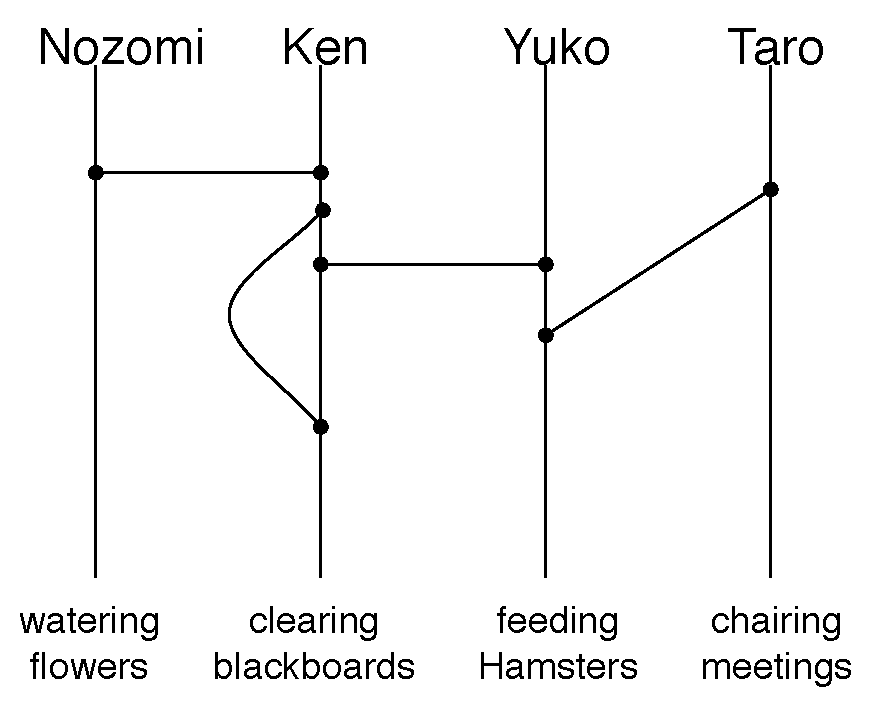
\includegraphics[scale=0.6]{amida.eps}
  \caption[An example of Amida lotteries.]{An example of Amida
  lotteries.  Nozomi clears blackboards; Ken waters flowers; Yuko chairs
  meetings; and Taro feeds Hamsters.}
  \label{amida-lottery}
 \end{figure}


\section{To the Next Chapters}

Each chapter can be read independently.
Chapter~\ref{ch:exchange} treats a synchronous hyper-lambda calculus and
Chapter~\ref{ch:lambda} deals with an asynchronous one.
The operational semantics is simpler in the synchronous case while
the type system is more exotic in the synchronous case.
The asynchronous one is apt for shared--memory implementation.
